\documentclass[
	12pt,				% tamanho da fonte
	%openright,			% capítulos começam em pág ímpar (insere página vazia caso preciso)
	%twoside,			% para impressão em recto e verso. Oposto a oneside
	openany,			%Para nao pular folhas quando um paragrafo novo começa. Oposto de Twoside e openright
	a4paper,			% tamanho do papel.
	chapter=TITLE,		% títulos de capítulos convertidos em letras maiúsculas
	section=TITLE,		% títulos de seções convertidos em letras maiúsculas
	%subsection=TITLE,	% títulos de subseções convertidos em letras maiúsculas
	%subsubsection=TITLE,% títulos de subsubseções convertidos em letras maiúsculas
	english,
	brazil				% o último idioma é o principal do documento
]{abntex2}
\usepackage[brazil]{babel}
\usepackage[utf8]{inputenc} %Pacote de linguas
\usepackage[normalem]{ulem}
\usepackage[T1]{fontenc}
\usepackage{lipsum}
\usepackage{cmap}
\usepackage{graphicx}
\usepackage[brazilian,hyperpageref]{backref}
\usepackage[alf]{abntex2cite} % Citações padrão ABNT
\usepackage{rotating}
\usepackage{float}
\usepackage{color}
\usepackage{listings}    
\usepackage{inconsolata}

\usepackage{listings}

\newcommand{\imagem}[3]{
	\begin{figure}[htb]
		\begin{center}
			\includegraphics[scale=0.5]{#1}
		\end{center}
		\caption{#2}	%\label{#3}
	\end{figure}
}

\title{Sistemas operacionais II \\ Lista de exercícios 7}
\date{\today}
\autor{Felipe Menino Carlos}

\setlength{\parindent}{1.3cm}
\frenchspacing

% Adicionando idioma
\selectlanguage{brazil}

\begin{document}
\maketitle

\chapter{Exercícios}

Os exercícios abaixo foram propostos pelo professor Gerson na aula de Sistemas operacionais, veja que, no caso dos exercícios com multiplas máquinas, foram utilizadas uma máquina física e uma virtual.

\subsection{Exercício 1}

Crie três arquivos de texto, com a extensão .txt, como segue:

Para a criação e edição dos arquivos foram usadas os comandos abaixo:
\begin{itemize}
	\item vim arquivo1.txt
	\item vim arquivo2.txt
	\item vim arquivo3.txt
	\item vim arquivo4.txt
\end{itemize}

O conteúdo de cada um dos arquivos, respectivamente, pode ser visto abaixo:

\begin{figure}[H]
  \centering
  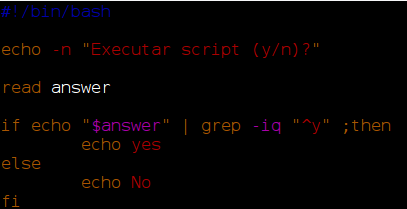
\includegraphics[scale=0.5]{arquivo1.png}
\end{figure}


\begin{figure}[H]
  \centering
  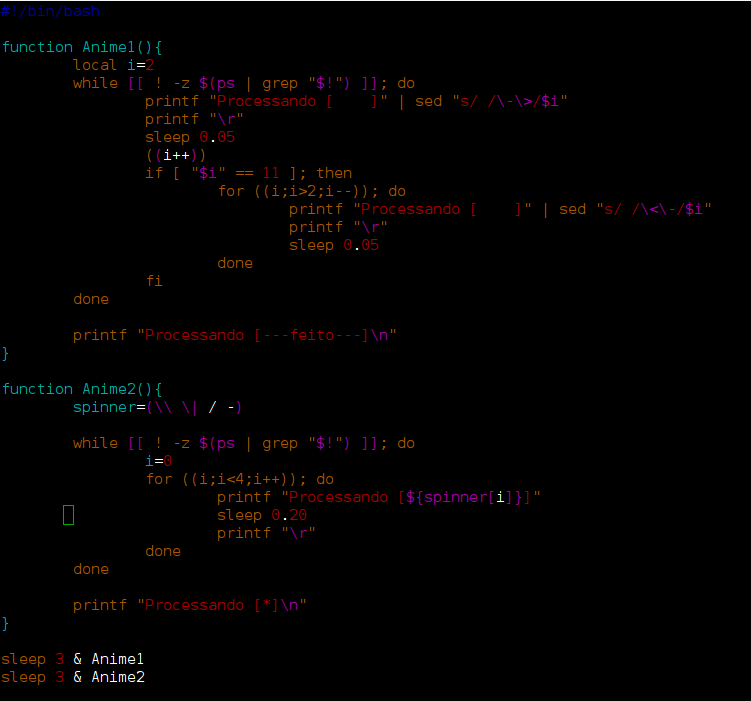
\includegraphics[scale=0.5]{arquivo2.png}
\end{figure}


\begin{figure}[H]
  \centering
  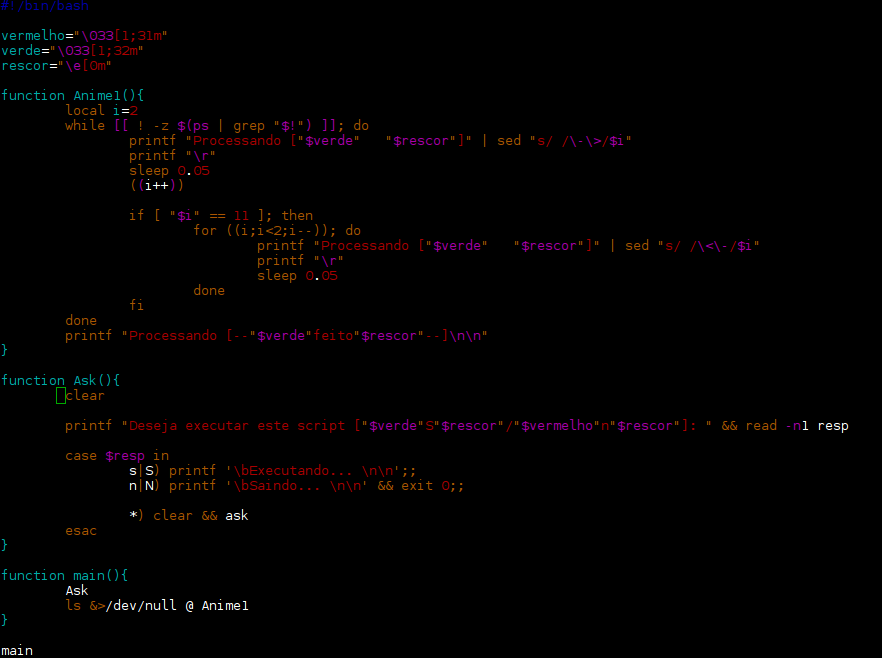
\includegraphics[scale=0.5]{arquivo3.png}
\end{figure}

\begin{figure}[H]
  \centering
  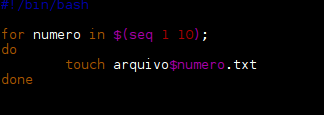
\includegraphics[scale=1]{arquivo4.png}
\end{figure}

\subsection{Exercício 2}

Transforme  os  arquivos  em  um  tarball  e  envie, por scp, para um  de  seus  colegas. Faça isso para as duas formas de compactação gzip e bzip.

Transformando em tarball e compactando
\begin{itemize}
\item GZip
	\begin{itemize}
		\item tar -cvzf scriptsOne.tar.gz arquivo1.txt arquivo2.txt arquivo3.txt arquivo4.txt 
	\end{itemize}

\item BZip
	\begin{itemize}
		\item tar -cvjf scriptsTwo.tar.bz arquivo1.txt arquivo2.txt arquivo3.txt arquivo4.txt 
	\end{itemize}
\end{itemize}

Após a criação dos arquivos \textbf{.bz} e \textbf{.gz} o seguite comando foi utilizado para fazer o envio dos arquivos para outra máquina
\begin{itemize}
	\item scp *.tar.* felipe@192.168.0.17
\end{itemize}

\subsection{Exercício 3}

Se  você foi  o  colega que  recebeu  o  arquivo. Tente  extrair  os  arquivos  do  tarball  e mude a extensão de .txt para .sh.

Movendo para um diretório somente para \textbf{gzip} e descompactando para \textbf{gzip}

\begin{itemize}
	\item mkdir gzip \&\& mv scriptsOne.tar.gz gzip \&\& cd gzip \&\& tar -xvzf scriptsOne.tar.gz
\end{itemize}

Após criar e descompactar, voltei para o diretório anterior

\begin{itemize}
	\item cd..

\end{itemize}

Movendo para um diretório somente \textbf{bzip} e descompactando
\begin{itemize}
	\item mkdir bzip \&\& mv scriptsTwo.tar.bz bzip \&\& cd bzip \&\& tar -xvjf scriptsTow.tar.gz
\end{itemize}

Mudando a extensão
\begin{itemize}
	\item mv arquivo1.txt arquivo1.sh ; mv arquivo2.txt arquivo2.sh ; mv arquivo3.txt arquivo3.sh ; mv arquivo4.txt arquivo4.sh
\end{itemize}

\subsection{Exercício 4}

Execute cada um dos arquivos .sh.


Dando permissão de execução
\begin{itemize}
	\item chmod +x *.sh
\end{itemize}

Executando os arquivos
\begin{itemize}
	\item./arquivo1.sh
	\item ./arquivo2.sh
	\item ./arquivo3.sh
	\item ./arquivo4.sh
\end{itemize}

\subsection{Exercício 5}

A execução do arquivo4 irá criar outros arquivos. Junte esses arquivos em um tarball e devolva ao seu colega usando o scp

\begin{itemize}
	\item tar -cvzf arquivosGerados.tar.gz *.txt
	\item scp arquivosGerados.tar.gz felipe@192.168.0.11:/home/felipe 
\end{itemize}

O resultado dos exercícios \textbf{4} e \textbf{5} podem ser visualizados abaixo

Resultados na máquina que recebeu e fez a execução dos scripts, e logo após devolveu para a máquina de origem
\begin{figure}[H]
  \centering
  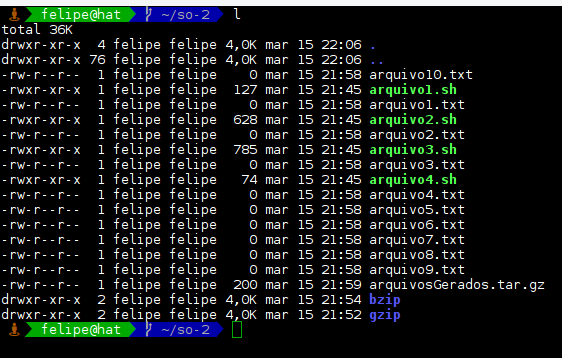
\includegraphics[scale=0.5]{resultados.png}
\end{figure}


Veja que na imagem mostrada acima, há os arquivos criados e os scripts que foram transferidos e descompactados.

Resultado na máquina de origem
\begin{figure}[H]
  \centering
  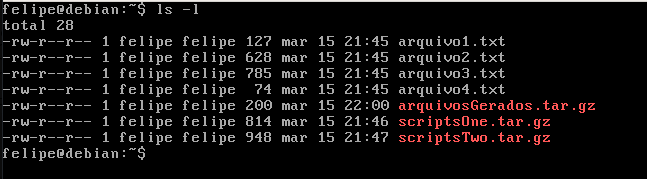
\includegraphics[scale=0.5]{result_server.png}
\end{figure}

Perceba que o arquivo \textbf{arquivosGerados.tar.gz} ficou também está na máquina de origem, e isto ocorre pois houve a transferência dos arquivos gerados no \textbf{exercício 5}


\end{document}	

